\documentclass{letter}

\usepackage{csquotes}
\usepackage[margin=1in]{geometry}
\usepackage{tikz}
\usepackage{amsmath}
\usepackage{enumitem}

\newcommand{\heading}[1]{{\large \textsc{#1}}}

\begin{document}

\heading{COMP 282 - Midterm 1 (Fall, 2018)}
\kern 2cm
\heading{Name:}

{\bf Question 1} \kern 1cm Provide a short answer to the following questions.

\begin{enumerate}[label=(\alph*)]

\item What is the benefit to using a binary tree over other data structures?

\vspace{3cm}

\item Give an example of when you would use a graph?

\vspace{3cm}

\item What is a clique?

\vspace{3cm}

\item What is one quality that {\em all} trees exhibit, that graphs, in
general, do not?

\vspace{3cm}

\item What is the balance property all {\em AVL Trees} seek to maintain?

\end{enumerate}

\clearpage

{\bf Question 2} \kern 1cm Build a proper {\em AVL Tree} given the following
inputs.  Show all steps.  Include -- at each step -- the balance factor of each
node.

\begin{verbatim} 3, 2, 1, 4, 5, 6 \end{verbatim}

\clearpage

{\bf Question 3} \kern 1cm Provide all of the listed traversals for the
following binary tree.  Be sure to label them.

\begin{itemize}
\item Pre-order traversal.
\item In-order traversal.
\item Breadth-first traversal.
\end{itemize}

\begin{center}
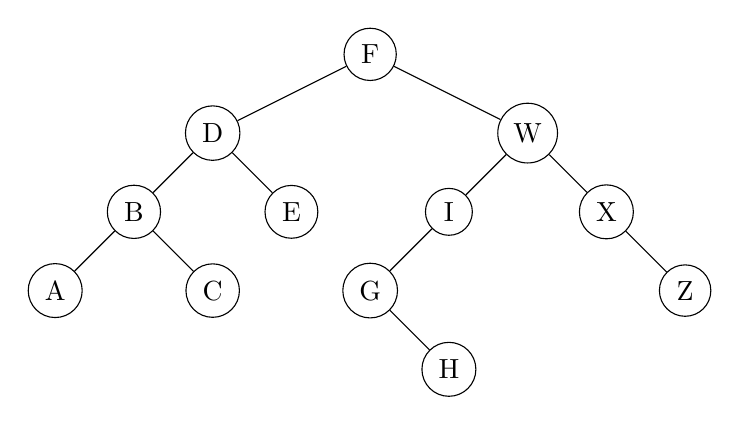
\begin{tikzpicture}
\node[shape=circle,draw=black] (F) at (1,0) {F};
\node[shape=circle,draw=black] (D) at (-1,-1) {D};
\node[shape=circle,draw=black] (B) at (-2,-2) {B};
\node[shape=circle,draw=black] (E) at (0,-2) {E};
\node[shape=circle,draw=black] (A) at (-3,-3) {A};
\node[shape=circle,draw=black] (C) at (-1,-3) {C};
\node[shape=circle,draw=black] (W) at (3,-1) {W};
\node[shape=circle,draw=black] (I) at (2,-2) {I};
\node[shape=circle,draw=black] (Y) at (4,-2) {X};
\node[shape=circle,draw=black] (Z) at (5,-3) {Z};
\node[shape=circle,draw=black] (G) at (1,-3) {G};
\node[shape=circle,draw=black] (H) at (2,-4) {H};

\path (F) edge (D);
\path (D) edge (B);
\path (D) edge (E);
\path (B) edge (A);
\path (B) edge (C);
\path (F) edge (W);
\path (W) edge (I);
\path (W) edge (Y);
\path (Y) edge (Z);
\path (I) edge (G);
\path (G) edge (H);
\end{tikzpicture}
\end{center}

\clearpage

{\bf Question 4} \kern 1cm Insert the value \texttt{5} into the following {\em
Red-Black Tree}.  Denote red nodes with a dashed outline, black nodes with a
solid circle, and double-black nodes with a double-solid circle.  Show all
steps.

\begin{center}
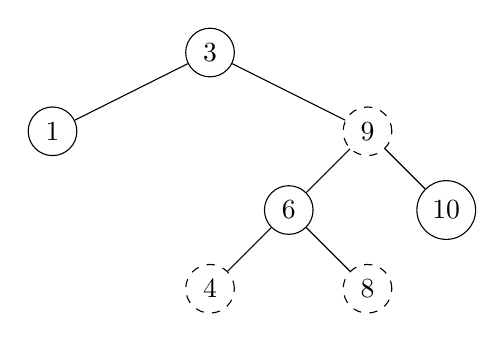
\begin{tikzpicture}
\node[shape=circle,draw=black] (3) at (0,0) {3};
\node[shape=circle,draw=black] (1) at (-2,-1) {1};
\node[shape=circle,draw=black,dashed] (9) at (2,-1) {9};
\node[shape=circle,draw=black] (6) at (1,-2) {6};
\node[shape=circle,draw=black,dashed] (4) at (0,-3) {4};
\node[shape=circle,draw=black,dashed] (8) at (2,-3) {8};
\node[shape=circle,draw=black] (10) at (3,-2) {10};

\path (3) edge (1);
\path (3) edge (9);
\path (9) edge (6);
\path (9) edge (10);
\path (6) edge (4);
\path (6) edge (8);
\end{tikzpicture}
\end{center}

\clearpage

{\bf Question 5} \kern 1cm Build a proper {\em 2-3-4 Tree} from the following
input.  Show all steps, including rotations.

\begin{verbatim}
insert 1,3,4,6
delete 3
insert 2, 7, 8, 9
delete 6
\end{verbatim}

\clearpage

{\bf Question 6} \kern 1cm Delete the \texttt{I} node from the following {\em
Red-Black Tree}.  Denote red nodes with a dashed outline, black nodes with a
solid circle, and double-black nodes with a double-solid circle.  Show all
steps.

\begin{center}
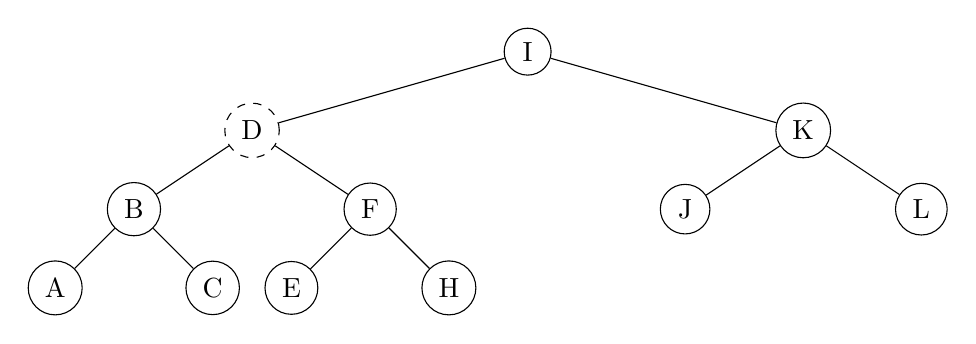
\begin{tikzpicture}
\node[shape=circle,draw=black] (I) at (0,0) {I};
\node[shape=circle,draw=black,dashed] (D) at (-3.5,-1) {D};
\node[shape=circle,draw=black] (B) at (-5,-2) {B};
\node[shape=circle,draw=black] (A) at (-6,-3) {A};
\node[shape=circle,draw=black] (C) at (-4,-3) {C};
\node[shape=circle,draw=black] (F) at (-2,-2) {F};
\node[shape=circle,draw=black] (E) at (-3,-3) {E};
\node[shape=circle,draw=black] (H) at (-1,-3) {H};
\node[shape=circle,draw=black] (K) at (3.5,-1) {K};
\node[shape=circle,draw=black] (J) at (2,-2) {J};
\node[shape=circle,draw=black] (L) at (5,-2) {L};

\path (I) edge (D);
\path (I) edge (K);
\path (D) edge (B);
\path (D) edge (F);
\path (K) edge (J);
\path (K) edge (L);
\path (B) edge (A);
\path (B) edge (C);
\path (F) edge (E);
\path (F) edge (H);
\end{tikzpicture}
\end{center}

\clearpage

{\bf Question 7} \kern 1cm Given the following adjacency matrix, draw the
weighted, undirected graph with $V = \{ v_0, v_1, v_2, v_3, v_4, v_5 \}$.

\begin{equation*}
\begin{bmatrix}
0 & 1 & 0 & 2 & 3 & 0 \\
0 & 0 & 4 & 1 & 0 & 2 \\
0 & 0 & 0 & 2 & 3 & 0 \\
0 & 0 & 0 & 0 & 1 & 4 \\
0 & 0 & 0 & 0 & 0 & 0 \\
0 & 0 & 0 & 0 & 0 & 0 \\
\end{bmatrix}
\end{equation*}

\clearpage

{\huge \textsc{No Illustrations}}

\vspace{1cm}

{\bf Question 8} \kern 1cm Given the following graph $G=(V,E)$, list the
vertices that form a connected component with $v_3$.

\begin{equation*}
V = \left \{ v_0, v_1, v_2, v_3, v_4, v_5, v_6, v_7, v_8, v_9 \right \}
\end{equation*}
\begin{equation*}
E = \left \{ \{ v_0, v_1 \}, \{ v_1, v_3 \}, \{ v_0, v_3 \}, \{ v_3, v_4 \}, \{ v_4, v_6 \}, \{ v_2, v_5 \}, \{ v_5, v_7 \}, \{ v_5, v_8 \}, \{ v_7, v_8 \}, \{ v_7, v_9 \}, \{ v_8, v_9 \} \right \}
\end{equation*}

\clearpage

{\huge \textsc{No Illustrations}}

\vspace{1cm}

{\bf Question 9} \kern 1cm Use Kruskal's Algorithm to calculate the minimum
spanning forest of the following graph $G = (V, E, w)$.  Show all steps.  List
all vertices in a particular spanning tree, and give its final cost.

\begin{equation*}
V = \left \{ v_0, v_1, v_2, v_3, v_4, v_5, v_6, v_7, v_8, v_9 \right \}
\end{equation*}

\begin{tabular}{ c | c }
E & w \\ \hline
$v_1,v_2$ & 1 \\
$v_1,v_4$ & 2.5 \\
$v_2,v_3$ & 1.5 \\
$v_5,v_0$ & 7 \\
$v_0,v_7$ & 0.2 \\
$v_6,v_3$ & 8.4 \\
$v_8,v_9$ & 2.6 \\
\end{tabular}

\clearpage

{\huge \textsc{No Illustrations}}

\vspace{1cm}

{\bf Question 10} \kern 1cm Given the graph $G = (V, E, w)$, below, find the
shortest path between $v_2$ and $v_6$.

\begin{equation*}
V = \{ v_0, v_1, v_2, v_3, v_4, v_5, v_6, v_7 \}
\end{equation*}

\begin{tabular}{ c | c }
E & w \\ \hline
$v_0,v_1$ & 0.5 \\
$v_0,v_3$ & 1.2 \\
$v_0,v_4$ & 0.3 \\
$v_1,v_2$ & 1.9 \\
$v_1,v_3$ & 2.2 \\
$v_1,v_5$ & 1.3 \\
$v_2,v_3$ & 4.7 \\
$v_2,v_7$ & 9.1 \\
$v_4,v_6$ & 2.7 \\
$v_5,v_6$ & 3.1 \\
$v_6,v_7$ & 2.8 \\
\end{tabular}

\end{document}
